\section{A physical collar of analytic caustics}\label{sec:caustics}

We now pass from the joint solution of the stationarity equation to
curves in the table. The essential point is that their support functions
move strictly inward to first order in the parameter \(\lambda=t^2\).
For phase-to-caustic correspondences under smoother initial foliations,
compare \citet[Section~2.7]{Glutsyuk2024}; the continuous phase leaves
here require the preceding graph and analytic regularization arguments.

\begin{proposition}\label{prop:physical-collar}
There exist \(\lambda_0>0\) and a jointly real-analytic family
\[
 \Gamma_\lambda:\T\longrightarrow\R^2,
 \qquad 0\leq\lambda\leq\lambda_0,
\]
with the following properties. The zero leaf parametrizes
\(\partial\Omega\); each positive leaf is a smooth, simple, regular,
strictly convex caustic contained in \(\Omega\); and the map
\[
 (\theta,b)\longmapsto\Gamma_{b\lambda_0}(\theta),
 \qquad (\theta,b)\in\T\times[0,1),
\]
is a homeomorphism onto a relatively open neighborhood of
\(\partial\Omega\) in \(\overline\Omega\).
Joint real analyticity here means extension to a neighborhood of the
closed parameter cylinder.
\end{proposition}

\begin{proof}
Let \(V\) be the function supplied by Theorem~\ref{thm:joint}, and set
\begin{equation}\label{phys:line-family}
 \Theta(y,t)=\phi(V(y,t)),\qquad
 p(y,t)=-\cS_1\bigl(\Theta(y,t),\Theta(y+t,t)\bigr).
\end{equation}
For real \(y,t\) sufficiently close to the zero-parameter circle,
\(\Theta_y>0\) and
\[
 \Theta(y+2\pi,t)=\Theta(y,t)+2\pi.
\]
The normalization in \eqref{eq:normalized-action} changes a chain action
only by a nonzero constant factor and a telescoping endpoint term.
Consequently, the equation in Theorem~\ref{thm:joint} gives
\begin{equation}\label{phys:stationarity}
 \cS_1\bigl(\Theta(y,t),\Theta(y+t,t)\bigr)
 +\cS_2\bigl(\Theta(y-t,t),\Theta(y,t)\bigr)=0.
\end{equation}
For sufficiently small \(t>0\), successive angles have positive small
increments. The generating relation for the actual billiard map and
\eqref{phys:stationarity}, shifted once in \(y\), therefore give
\begin{equation}\label{phys:invariance}
 T\bigl(\Theta(y,t),p(y,t)\bigr)
   =\bigl(\Theta(y+t,t),p(y+t,t)\bigr).
\end{equation}
In particular, these line states form an invariant graph, and the
invariance is onto: the parameter map is the circle translation
\(y\mapsto y+t\).

Both functions in \eqref{phys:line-family} are even in \(t\).
For \(\Theta\) this follows from the parity of \(V\). For \(p\), use
antisymmetry of \(\cS\) and \eqref{phys:stationarity}:
\begin{align*}
 p(y,-t)
 &=-\cS_1\bigl(\Theta(y,t),\Theta(y-t,t)\bigr)\\
 &=\cS_2\bigl(\Theta(y-t,t),\Theta(y,t)\bigr)
 =p(y,t).
\end{align*}
At \(t=0\), the generating relation gives \(p(y,0)=h(\Theta(y,0))\).
There is also a quantitative inward displacement. Put
\[
 a(y,t)=\frac{\Theta(y+t,t)-\Theta(y,t)}2.
\]
The line-coordinate formula of Section~\ref{sec:geometry}, expanded
at fixed \(\theta=\Theta(y,t)\), reads
\[
 p=h(\theta+a)\cos a-h'(\theta+a)\sin a
   =h(\theta)-\frac12r(\theta)a^2+O(a^3).
\]
Since \(a(y,t)=\frac12\Theta_y(y,0)t+O(t^2)\), and the displacement
\(h(\Theta)-p\) is even and analytic in \(t\), this implies
\begin{equation}\label{phys:inward-expansion}
 h(\Theta(y,t))-p(y,t)
 =\frac18r(\Theta(y,0))\Theta_y(y,0)^2t^2+O(t^4).
\end{equation}
The expansion and its derivatives are uniform on the real circle.

An even holomorphic function of \(t\) is holomorphic in
\(\lambda=t^2\) near zero, as is seen from its convergent power series.
Write the resulting functions as
\(\widehat\Theta(y,\lambda)\) and \(\widehat p(y,\lambda)\).
The analytic inverse function theorem, positivity of
\(\widehat\Theta_y\), and degree one give a jointly real-analytic angular
inverse \(y=Y(\theta,\lambda)\), with its natural \(2\pi\)-equivariance.
Compactness of the circle makes the parameter neighborhood uniform.
Define the periodic function
\[
 g(\theta,\lambda)=\widehat p(Y(\theta,\lambda),\lambda).
\]
It is the support candidate for the graph in \eqref{phys:invariance}.
In particular, \(g(\theta,0)=h(\theta)\). Substituting the angular
inverse in \eqref{phys:inward-expansion} gives, now at fixed \(\theta\),
\begin{equation}\label{phys:fixed-angle-expansion}
 g(\theta,\lambda)=h(\theta)-c(\theta)\lambda+O(\lambda^2),
 \qquad
 c(\theta)=\frac18r(\theta)
       \Theta_y(Y(\theta,0),0)^2>0.
\end{equation}
Thus no change of angle can remove the strict inward derivative.
Choose \(\lambda_0>0\) strictly inside the common analytic parameter
neighborhood. Decreasing it if necessary, we may arrange on the entire
closed cylinder \(0\leq\lambda\leq\lambda_0\) that
\begin{equation}\label{phys:support-inequalities}
 g>0,\qquad
 \rho:=g+g_{\theta\theta}>0,\qquad
 g_\lambda\leq-c_0<0,
\end{equation}
where \(c_0\) is a constant. The first two inequalities follow from
\(h>0\) and \(r=h+h''>0\), and the third from
\eqref{phys:fixed-angle-expansion}.

For each \(\lambda\) define
\begin{equation}\label{phys:body-and-boundary}
 \begin{split}
 K_\lambda
   &=\bigcap_{\theta\in\T}
       \{z\in\R^2:z\cdot n_\theta\leq g(\theta,\lambda)\},\\
 \Gamma_\lambda(\theta)
   &=g(\theta,\lambda)n_\theta
     +g_\theta(\theta,\lambda)e_\theta.
 \end{split}
\end{equation}
Figure~\ref{fig:phase-to-caustic} illustrates this construction: a point
of the line graph specifies a support line, and the formula for
$\Gamma_\lambda$ gives its contact point. We next verify that these
formal envelopes are the boundaries of the bodies $K_\lambda$.

\begin{figure}[t]
\centering
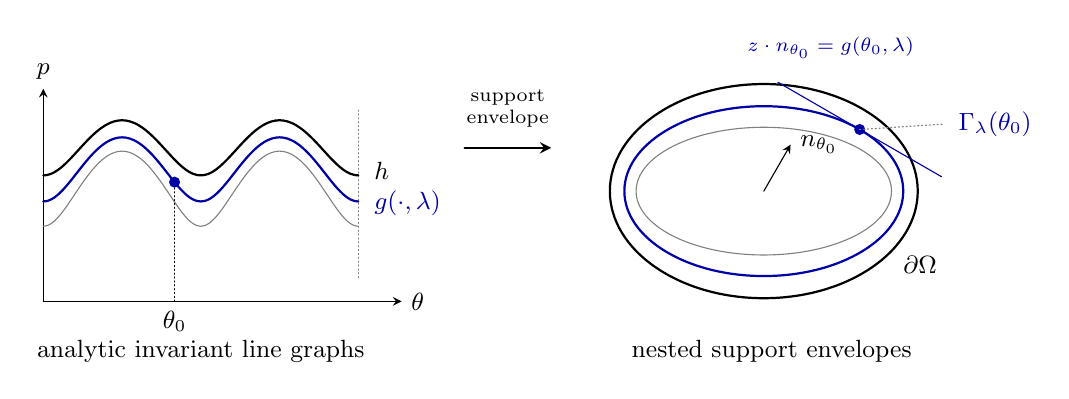
\begin{tikzpicture}[font=\small,>=stealth,line cap=round]
  \pgfmathsetmacro{\selectedsupport}{sqrt(4.34*cos(60)^2+1.61*sin(60)^2)}
  \pgfmathsetmacro{\contactx}{.85*4.34*cos(60)/\selectedsupport}
  \pgfmathsetmacro{\contacty}{.85*1.61*sin(60)/\selectedsupport}
  \begin{scope}
    \draw[->] (0,0)--(4.55,0) node[right] {$\theta$};
    \draw[->] (0,0)--(0,2.7) node[above] {$p$};
    \draw[densely dotted,gray] (4,.3)--(4,2.45);
    \draw[thick,domain=-90:270,samples=81,smooth,variable=\a]
      plot ({(\a+90)/90},{sqrt(5.29*cos(\a)^2+2.56*sin(\a)^2)});
    \draw[blue!65!black,thick,domain=-90:270,samples=81,smooth,variable=\a]
      plot ({(\a+90)/90},{sqrt(4.34*cos(\a)^2+1.61*sin(\a)^2)});
    \draw[gray,domain=-90:270,samples=81,smooth,variable=\a]
      plot ({(\a+90)/90},{sqrt(3.64*cos(\a)^2+.91*sin(\a)^2)});
    \node[anchor=west] at (4.08,1.66) {$h$};
    \node[anchor=west,blue!65!black] at (4.08,1.25) {$g(\cdot,\lambda)$};
    \draw[densely dotted] (1.6667,0)--(1.6667,\selectedsupport);
    \fill[blue!65!black] (1.6667,\selectedsupport) circle (2pt);
    \node[below] at (1.6667,0) {$\theta_0$};
    \node at (2,-.63) {analytic invariant line graphs};
  \end{scope}
  \draw[->,thick] (5.35,1.95)--(6.45,1.95);
  \node[align=center,font=\scriptsize] at (5.9,2.45) {support\\envelope};
  \begin{scope}[xshift=9.15cm,yshift=1.4cm]
    \draw[thick] (0,0) ellipse [x radius=1.955,y radius=1.36];
    \draw[blue!65!black,thick] (0,0)
      ellipse [x radius=1.77076,y radius=1.07853];
    \draw[gray] (0,0) ellipse [x radius=1.62173,y radius=.81086];
    \draw[blue!65!black]
      ({\contactx-1.2*cos(150)},{\contacty-1.2*sin(150)})--
      ({\contactx+1.2*cos(150)},{\contacty+1.2*sin(150)});
    \fill[blue!65!black] (\contactx,\contacty) circle (2pt);
    \draw[gray,thin,densely dotted] (\contactx,\contacty)--(2.27,.85);
    \node[anchor=west,blue!65!black] at (2.35,.85)
      {$\Gamma_\lambda(\theta_0)$};
    \node[anchor=south,blue!65!black,font=\scriptsize] at (.85,1.56)
      {$z\cdot n_{\theta_0}=g(\theta_0,\lambda)$};
    \draw[->] (0,0)--(.34,.59) node[right] {$n_{\theta_0}$};
    \node[anchor=west] at (1.65,-.93) {$\partial\Omega$};
    \node at (.1,-2.03) {nested support envelopes};
  \end{scope}
\end{tikzpicture}
\caption{The support-envelope correspondence, drawn schematically.
The highlighted point of $p=g(\theta,\lambda)$ specifies the blue
tangent line on the right; its contact point is
$\Gamma_\lambda(\theta_0)=g n_{\theta_0}+g_\theta e_{\theta_0}$,
with $g$ and $g_\theta$ evaluated at $(\theta_0,\lambda)$.
Positive $g+g_{\theta\theta}$ makes each envelope strictly convex,
and $g_\lambda<0$ makes the family strictly nested.}
\label{fig:phase-to-caustic}
\end{figure}


Each \(K_\lambda\) is a compact convex body with nonempty interior:
it contains a disk about the origin of radius
\(\min_\theta g(\theta,\lambda)>0\), and the constraint with normal
\(z/|z|\) bounds \(|z|\) by \(\max_\theta g(\theta,\lambda)\).
Moreover \(K_0=\overline\Omega\), by the definition of \(h\).

We verify directly that \(\Gamma_\lambda\) is the whole boundary and
has support function \(g(\cdot,\lambda)\). Differentiation gives
\begin{equation}\label{phys:normal-parametrization}
 \Gamma_\lambda'(\theta)=\rho(\theta,\lambda)e_\theta.
\end{equation}
For a fixed angle \(\alpha\),
\[
 \frac{\dd}{\dd\theta}
   \bigl(\Gamma_\lambda(\theta)\cdot n_\alpha\bigr)
 =\rho(\theta,\lambda)\sin(\alpha-\theta).
\]
This projection has its unique maximum, modulo \(2\pi\), at
\(\theta=\alpha\), where its value is \(g(\alpha,\lambda)\).
Hence every point \(\Gamma_\lambda(\theta)\) satisfies all the
constraints defining \(K_\lambda\), with equality for its own normal,
and belongs to \(\partial K_\lambda\).

Conversely, let \(z\in\partial K_\lambda\).
The continuous nonnegative function
\(g(\theta,\lambda)-z\cdot n_\theta\) must vanish somewhere: a positive
minimum would place a disk about \(z\) inside \(K_\lambda\).
At a zero \(\alpha\), its derivative also vanishes. Thus
\[
 z\cdot n_\alpha=g(\alpha,\lambda),\qquad
 z\cdot e_\alpha=g_\theta(\alpha,\lambda),
\]
which gives \(z=\Gamma_\lambda(\alpha)\).
The unique-maximum property proves that this parametrization is
one-to-one on \(\T\); \eqref{phys:normal-parametrization} makes it
regular. Each support line has exactly one contact point, so the
boundary contains no nontrivial line segment and the body is strictly
convex. In fact its curvature is \(1/\rho>0\).
All these curves are real analytic.

The last inequality in \eqref{phys:support-inequalities} gives, for
\(0\leq\lambda<\mu\leq\lambda_0\),
\[
 g(\theta,\mu)\leq g(\theta,\lambda)-c_0(\mu-\lambda)
 \quad\hbox{for every }\theta.
\]
It follows that \(K_\mu\) is contained in the interior of \(K_\lambda\),
with a uniform positive gap between them. In particular the boundaries
are pairwise disjoint, and \(\Gamma_\lambda\subset\Omega\) for
\(\lambda>0\).

The positively oriented tangent at \(\Gamma_\lambda(\theta)\) has
velocity \(e_\theta\) and line equation
\(z\cdot n_\theta=g(\theta,\lambda)\).
For \(\lambda>0\) these are precisely the line states in
\eqref{phys:invariance}, with \(t=\sqrt\lambda\).
They meet \(\Omega\), because their contact points lie in its interior.
The onto invariance in \eqref{phys:invariance} therefore preserves
tangency under both \(T\) and \(T^{-1}\). It supplies the tangent
successor segment at the forward endpoint and the tangent predecessor
segment at the back endpoint. Reflection is a linear involution:
if \(v'\) is the reflection of \(v\), then \(-v\) is the reflection
of \(-v'\). Reversing each such pair of segments proves tangency
preservation for the opposite orientation as well. Thus every positive
leaf is a smooth closed convex caustic, with the required reflection
property at either endpoint.

It remains to show that these curves fill a physical collar.
The map
\[
 F:\T\times[0,\lambda_0]\longrightarrow\overline\Omega,
 \qquad F(\theta,\lambda)=\Gamma_\lambda(\theta),
\]
is continuous and injective, by simplicity of the curves and strict
nesting. Since its domain is compact, it is a homeomorphism onto its
image. Set
\[
 A=K_0\setminus K_{\lambda_0}.
\]
This is relatively open in \(K_0=\overline\Omega\) and contains
\(\partial\Omega\). All leaves with \(\lambda<\lambda_0\) lie in \(A\).
For the converse, fix \(z\in A\) and consider its minimum support slack
\[
 m_z(\lambda)
   =\min_{\theta\in\T}
      \bigl(g(\theta,\lambda)-z\cdot n_\theta\bigr).
\]
This function is continuous, satisfies
\(m_z(0)\geq0>m_z(\lambda_0)\), and obeys
\[
 m_z(\mu)\leq m_z(\lambda)-c_0(\mu-\lambda)
 \qquad(\mu>\lambda).
\]
It has exactly one zero in \([0,\lambda_0)\).
At that zero, \(z\in\partial K_\lambda\), hence
\(z=\Gamma_\lambda(\theta)\) for exactly one \(\theta\).
The restriction of \(F\) to \(\T\times[0,\lambda_0)\) is therefore a
homeomorphism onto \(A\). Rescaling \(\lambda=b\lambda_0\) completes
the proof.
\end{proof}

\begin{proof}[Proof of Theorem~\ref{thm:collar-regularity}]
Theorem~\ref{thm:analytic-boundary} proves that the billiard boundary
is real analytic. Theorem~\ref{thm:joint} and
Proposition~\ref{prop:physical-collar} give the asserted jointly
real-analytic family of strictly convex caustics and its full
physical collar.
\end{proof}

\begin{proof}[Proof of Theorem~\ref{thm:main}]
Proposition~\ref{prop:physical-collar} gives exactly the continuous
caustic collar of \cite[Definition~1.1]{NB}: the boundary is the zero
leaf, the positive leaves are smooth closed convex caustics, and the
family parametrizes a relatively open neighborhood of the boundary
in the closed table. The original assumptions supply the remaining
smoothness, strict convexity, and positive curvature hypotheses.
Theorem~\ref{thm:nb-rigidity}, namely \cite[Theorem~1.2]{NB},
therefore implies that \(\Omega\) is an ellipse. Undoing the initial
translation gives a center \(c\in\R^2\) and a real symmetric
positive-definite matrix \(Q\) with
\[
 \Omega=\{x\in\R^2:(x-c)^TQ(x-c)<1\},
\]
as required.
\end{proof}
